\chapter{Сложные структуры данных}
\label{ch:advanced-ds}

\section{Красно-чёрные деревья}
\label{sec:rb-tree}
Красно-чёрное дерево представляет собой бинарное дерево поиска с одним дополнительным битом \emph{цвета}. Цвет узла может быть либо красным, либо чёрным. В соответствии с накладываемыми на узлы дерева ограничениями, ни один путь в красно-чёрном дереве не отличается от другого по длине более чем в два раза, что делает его сбалансированным. Вот эти ограничения:
\begin{enumerate}
  \item Корень дерева является чёрным.
  \item Красный узел может быть потомком только чёрного узла.
  \item Все пути от корня к пустым узлам содержат одинаковое количество чёрных узлов.
  \item Пустой узел — чёрный.
\end{enumerate}

\subsection{Реализация}
При вставке нового узла в дерево может возникнуть одна из четырёх ситуаций, представленных на рисунке, когда красный узел является потомком тоже красного узла. На этом же рисунке показаны необходимые преобразования, чтобы дерево вновь стало сбалансированным.

\begin{figure}[t]
  \centering
  \begin{tikzpicture}[red/.style={circle,draw},
                      black/.style={circle,draw,fill=gray},
                      level distance=1cm,
                      font=\footnotesize]
    \node [black] at (0,0) {$z$}
      child { node [red] {$x$}
        child { node [] {$a$} }
        child { node [red] {$y$}
          child { node [] {$b$} }
          child { node [] {$c$} } } }
      child { node [] {$d$} };

    \node [black] at (-4,-4.5) {$z$}
      child { node [red] {$y$}
        child { node [red] {$x$}
          child { node [] {$a$} }
          child { node [] {$b$} } }
        child { node [] {$c$} } }
      child { node [] {$d$} };

    \node [black] at (4,-4.5) {$x$}
      child { node [] {$a$} }
      child { node [red] {$y$}
        child { node [] {$b$} }
        child { node [red] {$z$}
          child { node [] {$c$} }
          child { node [] {$d$} } } };

    \node [black] at (0,-8.5) {$x$}
      child { node [] {$a$} }
      child { node [red] {$z$}
        child { node [red] {$y$}
          child { node [] {$b$} }
          child { node [] {$c$} } }
        child { node [] {$d$} } };


    \begin{scope}[level/.style={sibling distance=11mm/#1}]
      \node [red] at (0,-4.5) {$y$}
        child { node [black] {$x$}
          child { node [] {$a$} }
          child { node [] {$b$} } }
        child { node [black] {$z$}
          child { node [] {$c$} }
          child { node [] {$d$} } };
    \end{scope}

    \draw [->,thick] (-2.5,-5.5) -- (-1.5,-5.5);
    \draw [->,thick] (2.5,-5.5) -- (1.5,-5.5);
    \draw [->,thick] (0,-3.2) -- (0,-4);
    \draw [->,thick] (0,-7.8) -- (0,-7);
  \end{tikzpicture}
  \caption{Балансировка дерева}
\end{figure}

\lstinputlisting[style=ocamlstyle,caption=Реализация красно-чёрного дерева]{src/advanced-ds/rbtree.ml}

\section{Префиксные деревья}
\label{sec:trie}
Префиксное дерево (trie) — структура данных, позволяющая хранить ассоциативный массив, ключами которого являются, как правило, строки. В отличие от двоичных деревьев поиска не обязательно хранить ключ в узлах дерева, так как в префиксном дереве по позиции узла можно вычислить ключ, ассоциированный с ним. Все потомки узла имеют общий префикс, представленный этим самым узлом.

Ниже на рисунке представлено префиксное дерево с некоторыми английскими словами в качестве ключей.
\begin{center}
  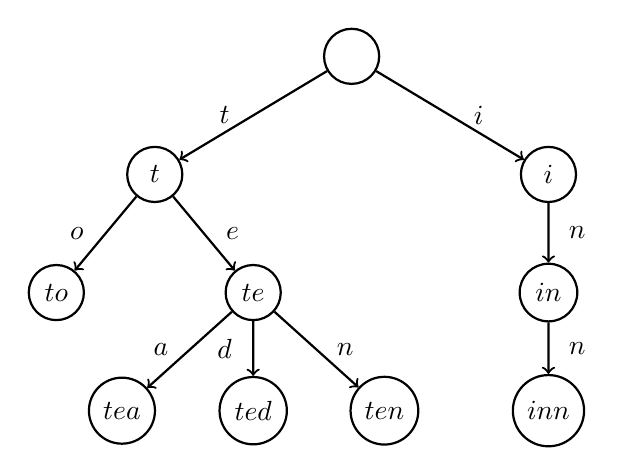
\begin{tikzpicture}[minimum size=7mm,
                      circle,thick,
                      edge from parent/.style={->,draw,thick},
                      level/.style={sibling distance=50mm/#1}]
    \node [draw] {}
      child { node [draw] {$t$}
        child { node [draw] {$to$}
          edge from parent
            node[left] {$o$}
        }
        child { node [draw] {$te$}
          child { node [draw] {$tea$}
            edge from parent
              node[left] {$a$}
          }
          child { node [draw] {$ted$}
            edge from parent
              node[left] {$d$}
          }
          child { node [draw] {$ten$}
            edge from parent
              node[right] {$n$}
          }
          edge from parent
            node[right] {$e$}
        }
        edge from parent
          node[left] {$t$}
      }
      child { node [draw] {$i$}
        child { node [draw] {$in$}
          child { node [draw] {$inn$}
            edge from parent
              node[right] {$n$}
          }
          edge from parent
            node[right] {$n$}
        }
        edge from parent
          node[right] {$i$}
      };
  \end{tikzpicture}
\end{center}

В качестве ключей могут использоваться не только строки, но и любая последовательность. Время вставки, удаления и поиска в префиксном дереве равно $O(m)$, где $m$ — длина ключа.

\lstinputlisting[style=ocamlstyle,caption=Реализация префиксного дерева]{src/advanced-ds/trie.ml}

\begin{ocamllst}{Пример использования}{}
# let root = empty
# let root = insert (String.to_list "tea") "tea" root
# let root = insert (String.to_list "ted") "ted" root
# let root = insert (String.to_list "ten") "ten" root
# let root = insert (String.to_list "inn") "inn" root
# let root = insert (String.to_list "te") "te" root
# let root = insert (String.to_list "") "" root ;;
value root : trie string char = {value=Some ""; children=<abstr>}

# let root = remove (String.to_list "") root
# let root = remove (String.to_list "te") root
# let root = remove (String.to_list "inn") root
# let root = remove (String.to_list "ten") root
# let root = remove (String.to_list "ted") root
# let root = remove (String.to_list "tea") root ;;
value root : trie string char = {value=None; children=<abstr>}

# Map.is_empty root.children ;;
- : bool = True
\end{ocamllst}

\section{Фильтр Блума}
\label{sec:bloom-filter}
Фильтр Блума (Bloom filter) — вероятностная структура данных, позволяющая компактно хранить информацию о принадлежности элемента множеству. Но при этом возможно \emph{ложноположительное сработывание}, то есть элемент в множестве не присутствует действительно, но согласно фильтру он там есть.

Фильтр Блума может использовать любой заданный объём памяти, причём чем он больше, тем меньше вероятность ложноположительного срабатывания. Эта структура данных поддерживает операцию добавления нового элемента в множество и операцию проверки присутствия элемента в множестве. С увеличением количества хранимых элементов повышается вероятность ложноположительного срабатывания.

Фильтр Блума состоит из битовой карты размером $m$ и хеш-функций $h_1,...,h_k$, которые задает пользователь. Изначально все биты равны нулю. Хеш-функции должны быть независимыми и распределены равномерно.

Для добавления элемента $e$ необходимо выставить биты в битовой карте в единицу на позициях $h_1(e),...,h_k(e)$.

Для проверки принадлежности элемента множеству, необходимо проверить биты на позициях $h_1(e),...,h_k(e)$. Если хотя бы один бит равен нулю, то элемент не принадлежит множеству. Если же все биты равны единице, то элемент \emph{возможно} принадлежит множеству.

\subsection{Вероятность ложноположительного срабатывания}
Пусть хеш-функции — незивисимы и распределены равномерно, то есть выбор любой позиции по значению хеш-функции — равновероятен, и $m$ — размер битовой карты. Тогда вероятность того, что какой-то определенный бит не будет установлен данной хеш-функцией, когда добавляется элемент в множество:
\[
1 - \frac{1}{m}.
\]

Вероятность, что этот бит не будет установлен ни одной хеш-функцией, равна:
\[
\left( 1 - \frac{1}{m} \right)^k.
\]

После вставки $n$ элементов, вероятность, что данный бит все ещё равен нулю:
\[
\left( 1 - \frac{1}{m} \right)^{nk}.
\]

В таком случае верояность, что он равен единице:
\[
1 - \left( 1 - \frac{1}{m} \right)^{nk}.
\]

Пусть мы теперь пробуем проверить принадлежность элемента, который мы не добавляли в фильтр. Тогда вероятность ложноположительного срабатывания будет равна:
\[
f= \left( 1 - \left[ 1 - \frac{1}{m} \right]^{nk} \right)^k =  \left( 1 - e^{-nk / m} \right)^k,
\]
используя второй замечательный предел\footnote{$\lim_{x \to \infty} \left( 1 + \frac{1}{x} \right)^x = e$}. Из этого следует, что при уменьшении размера $m$ и увеличинии $n$ увеличивается вероятность ложноположительного срабатывания. Для того, чтобы найти оптимальное количество $k$ хеш-функций, при котором вероятность ложноположительного срабатывания будет минимальной при фиксированных $m$ и $n$, следует взять производную $f$ по $k$. Для удобства взятия производной представим $f$ следующим образом:
\[
f = e^{k\ln(1 - e^{-nk / m})}.
\]

Пусть $g = k\ln(1 - e^{-nk / m})$. Тогда производная равна:
\[
\frac{\partial g}{\partial k} = ln(1 - e^{-nk / m}) + \frac{nk}{m} \frac{e^{-nk / m}}{1 - e^{-nk / m}}
\]

Производная $g$ равна нулю при $k = \ln 2 \cdot (m / n) \simeq 0.6931 \frac{m}{n}$. При этом вероятность ложноположительного срабатывания $f = (1 / 2)^k \simeq 0.6185^{m / n}$.

\subsection{Реализация}
\lstinputlisting[style=ocamlstyle]{src/advanced-ds/bloom.ml}

\begin{ocamllst}{Пример использования}{}
# let size = 18
# let hasher' = Hashtbl.hash
# let hasher'' x = abs ((Hashtbl.hash x) + (size / 2))
# let bloom = create [hasher'; hasher''] size
value bloom : bloom_filter '_a =
  {hashers=[<fun>; <fun>]; bitset=<abstr>; size=18}

# let bloom = insert "foo" bloom ;;
# BitSet.print stdout bloom.bitset; print_newline () ;;
100000000100000000000000

# let bloom = insert "bar" bloom ;;
# BitSet.print stdout bloom.bitset; print_newline () ;;
100100000100100000000000

# mem "foo" bloom ;;
- : bool = True
# mem "baz" bloom ;;
- : bool = False
\end{ocamllst}
